\documentclass[12pt,]{article}
\usepackage{lmodern}
\usepackage{amssymb,amsmath}
\usepackage{ifxetex,ifluatex}
\usepackage{fixltx2e} % provides \textsubscript
\ifnum 0\ifxetex 1\fi\ifluatex 1\fi=0 % if pdftex
  \usepackage[T1]{fontenc}
  \usepackage[utf8]{inputenc}
\else % if luatex or xelatex
  \ifxetex
    \usepackage{mathspec}
  \else
    \usepackage{fontspec}
  \fi
  \defaultfontfeatures{Ligatures=TeX,Scale=MatchLowercase}
\fi
% use upquote if available, for straight quotes in verbatim environments
\IfFileExists{upquote.sty}{\usepackage{upquote}}{}
% use microtype if available
\IfFileExists{microtype.sty}{%
\usepackage{microtype}
\UseMicrotypeSet[protrusion]{basicmath} % disable protrusion for tt fonts
}{}
\usepackage[margin=1in]{geometry}
\usepackage{hyperref}
\hypersetup{unicode=true,
            pdftitle={Logistic Regression},
            pdfauthor={Jose Luis Contreras Santos, Antonio Javier González Ferrer, Alejandro González Pérez},
            pdfkeywords={pandoc, r markdown, knitr},
            pdfborder={0 0 0},
            breaklinks=true}
\urlstyle{same}  % don't use monospace font for urls
\usepackage{natbib}
\bibliographystyle{plainnat}
\usepackage{color}
\usepackage{fancyvrb}
\newcommand{\VerbBar}{|}
\newcommand{\VERB}{\Verb[commandchars=\\\{\}]}
\DefineVerbatimEnvironment{Highlighting}{Verbatim}{commandchars=\\\{\}}
% Add ',fontsize=\small' for more characters per line
\usepackage{framed}
\definecolor{shadecolor}{RGB}{248,248,248}
\newenvironment{Shaded}{\begin{snugshade}}{\end{snugshade}}
\newcommand{\KeywordTok}[1]{\textcolor[rgb]{0.13,0.29,0.53}{\textbf{{#1}}}}
\newcommand{\DataTypeTok}[1]{\textcolor[rgb]{0.13,0.29,0.53}{{#1}}}
\newcommand{\DecValTok}[1]{\textcolor[rgb]{0.00,0.00,0.81}{{#1}}}
\newcommand{\BaseNTok}[1]{\textcolor[rgb]{0.00,0.00,0.81}{{#1}}}
\newcommand{\FloatTok}[1]{\textcolor[rgb]{0.00,0.00,0.81}{{#1}}}
\newcommand{\ConstantTok}[1]{\textcolor[rgb]{0.00,0.00,0.00}{{#1}}}
\newcommand{\CharTok}[1]{\textcolor[rgb]{0.31,0.60,0.02}{{#1}}}
\newcommand{\SpecialCharTok}[1]{\textcolor[rgb]{0.00,0.00,0.00}{{#1}}}
\newcommand{\StringTok}[1]{\textcolor[rgb]{0.31,0.60,0.02}{{#1}}}
\newcommand{\VerbatimStringTok}[1]{\textcolor[rgb]{0.31,0.60,0.02}{{#1}}}
\newcommand{\SpecialStringTok}[1]{\textcolor[rgb]{0.31,0.60,0.02}{{#1}}}
\newcommand{\ImportTok}[1]{{#1}}
\newcommand{\CommentTok}[1]{\textcolor[rgb]{0.56,0.35,0.01}{\textit{{#1}}}}
\newcommand{\DocumentationTok}[1]{\textcolor[rgb]{0.56,0.35,0.01}{\textbf{\textit{{#1}}}}}
\newcommand{\AnnotationTok}[1]{\textcolor[rgb]{0.56,0.35,0.01}{\textbf{\textit{{#1}}}}}
\newcommand{\CommentVarTok}[1]{\textcolor[rgb]{0.56,0.35,0.01}{\textbf{\textit{{#1}}}}}
\newcommand{\OtherTok}[1]{\textcolor[rgb]{0.56,0.35,0.01}{{#1}}}
\newcommand{\FunctionTok}[1]{\textcolor[rgb]{0.00,0.00,0.00}{{#1}}}
\newcommand{\VariableTok}[1]{\textcolor[rgb]{0.00,0.00,0.00}{{#1}}}
\newcommand{\ControlFlowTok}[1]{\textcolor[rgb]{0.13,0.29,0.53}{\textbf{{#1}}}}
\newcommand{\OperatorTok}[1]{\textcolor[rgb]{0.81,0.36,0.00}{\textbf{{#1}}}}
\newcommand{\BuiltInTok}[1]{{#1}}
\newcommand{\ExtensionTok}[1]{{#1}}
\newcommand{\PreprocessorTok}[1]{\textcolor[rgb]{0.56,0.35,0.01}{\textit{{#1}}}}
\newcommand{\AttributeTok}[1]{\textcolor[rgb]{0.77,0.63,0.00}{{#1}}}
\newcommand{\RegionMarkerTok}[1]{{#1}}
\newcommand{\InformationTok}[1]{\textcolor[rgb]{0.56,0.35,0.01}{\textbf{\textit{{#1}}}}}
\newcommand{\WarningTok}[1]{\textcolor[rgb]{0.56,0.35,0.01}{\textbf{\textit{{#1}}}}}
\newcommand{\AlertTok}[1]{\textcolor[rgb]{0.94,0.16,0.16}{{#1}}}
\newcommand{\ErrorTok}[1]{\textcolor[rgb]{0.64,0.00,0.00}{\textbf{{#1}}}}
\newcommand{\NormalTok}[1]{{#1}}
\usepackage{graphicx,grffile}
\makeatletter
\def\maxwidth{\ifdim\Gin@nat@width>\linewidth\linewidth\else\Gin@nat@width\fi}
\def\maxheight{\ifdim\Gin@nat@height>\textheight\textheight\else\Gin@nat@height\fi}
\makeatother
% Scale images if necessary, so that they will not overflow the page
% margins by default, and it is still possible to overwrite the defaults
% using explicit options in \includegraphics[width, height, ...]{}
\setkeys{Gin}{width=\maxwidth,height=\maxheight,keepaspectratio}
\IfFileExists{parskip.sty}{%
\usepackage{parskip}
}{% else
\setlength{\parindent}{0pt}
\setlength{\parskip}{6pt plus 2pt minus 1pt}
}
\setlength{\emergencystretch}{3em}  % prevent overfull lines
\providecommand{\tightlist}{%
  \setlength{\itemsep}{0pt}\setlength{\parskip}{0pt}}
\setcounter{secnumdepth}{0}
% Redefines (sub)paragraphs to behave more like sections
\ifx\paragraph\undefined\else
\let\oldparagraph\paragraph
\renewcommand{\paragraph}[1]{\oldparagraph{#1}\mbox{}}
\fi
\ifx\subparagraph\undefined\else
\let\oldsubparagraph\subparagraph
\renewcommand{\subparagraph}[1]{\oldsubparagraph{#1}\mbox{}}
\fi

%%% Use protect on footnotes to avoid problems with footnotes in titles
\let\rmarkdownfootnote\footnote%
\def\footnote{\protect\rmarkdownfootnote}

%%% Change title format to be more compact
\usepackage{titling}

% Create subtitle command for use in maketitle
\newcommand{\subtitle}[1]{
  \posttitle{
    \begin{center}\large#1\end{center}
    }
}

\setlength{\droptitle}{-2em}
  \title{Logistic Regression}
  \pretitle{\vspace{\droptitle}\centering\huge}
  \posttitle{\par}
  \author{Jose Luis Contreras Santos, Antonio Javier González Ferrer, Alejandro
González Pérez}
  \preauthor{\centering\large\emph}
  \postauthor{\par}
  \predate{\centering\large\emph}
  \postdate{\par}
  \date{enero, 2017}

\usepackage{bm}

\begin{document}
\maketitle
\begin{abstract}
A logistic regression project to determine the type of wine depending on
its physicochemical attributes.
\end{abstract}

\section{Introduction}\label{introduction}

Oh!, a wine factory is going to receive a new pack of different wines
and they do not have their type labelled (red or white). Ok, don't
worry, we can go through each of the wines, look at it color, and label
it. But\ldots{} we would like to do this process automatically. In the
following lines, we will face a classification problem to predict if the
wine is red or white, depending on its physicochemical attributes.

A classification problem relates input variables \(x\) to the output
variable \(y\), but now \(y\) can take only discrete values, instead of
continuous variables as in regression. When \(y\) can only take two
discrete, it is called binary classification. We will denote these
values as \(y \in \{0, 1\}\) in the rest of the report, where
\(0 \equiv\) white class and \(1 \equiv\) red type.

\section{Loading the data}\label{loading-the-data}

The data science pipeline often\footnote{Some statistical learning
  models are robust enough to do not need this division. They can infer
  the behaviour of the whole population from a sample if some
  statistical hypothesis are fulfilled.} needs to split the original
dataset into two smaller pieces: the train and test datasets. If we only
evaluate our models in the same dataset, the results will be
overestimated (aka overfitting). To provide honest assesments of the
performance of the predictive models, we will need to validate the
models using a test dataset, a partition that has not been used to build
the models in order to avoid bias.

\begin{Shaded}
\begin{Highlighting}[]
\CommentTok{# Loading the dataset into a dataframe}
\NormalTok{df <-}\StringTok{ }\KeywordTok{read_delim}\NormalTok{(}\StringTok{"../../data/processed/wines.csv"}\NormalTok{, }
  \StringTok{";"}\NormalTok{, }
  \DataTypeTok{escape_double =} \OtherTok{FALSE}\NormalTok{, }
  \DataTypeTok{trim_ws =} \OtherTok{TRUE}\NormalTok{)}

\CommentTok{# Train and test dataset, split 80%.}
\NormalTok{split =}\StringTok{ }\KeywordTok{nrow}\NormalTok{(df)*}\FloatTok{0.8}
\NormalTok{train =}\StringTok{ }\NormalTok{df[}\DecValTok{1}\NormalTok{:split,]}
\NormalTok{test =}\StringTok{ }\NormalTok{df[split:}\KeywordTok{nrow}\NormalTok{(df),]}
\end{Highlighting}
\end{Shaded}

In this case, the test dataset consists of the 20\% of the dataset (1300
observations).

\section{Logistic Regression Model}\label{logistic-regression-model}

The equivalent linear regression model in classification is the logistic
regression model. This model needs to specify a function such that
\(p(y=0|\bm{\tilde{X}})\) and \(p(y=1|\bm{\tilde{X}})\) are both greater
than 0 and sum 1. The logistic function has such properties, definining
the following model:

\[ p(y|\bm{\tilde{X}},\bm{\beta}) = \frac{e^{\bm{\beta} \bm{\tilde{X}}}}{1+e^{\bm{\beta} \bm{\tilde{X}}}} \]

If \(\beta_i > 0\) then increasing one unit in \(x_i\) will increase the
probability of a success. If \(\beta_i < 0\), then the probabilty of
success decrease when increasing \(x_i\). When \(\beta_i = 0\) ,
\(e^0 = 1\), so the odds do not change with \(x_i\).

\subsection{Full model}\label{full-model}

We start by defining a logistic regression model with all the 11
attributes as the predictors. We do not use the \texttt{quality}, used
in regression, and neither the \texttt{type}, used as the target
variable:

\begin{Shaded}
\begin{Highlighting}[]
\CommentTok{# Logistic regression model with all the variables.}
\NormalTok{log.full=}\KeywordTok{glm}\NormalTok{(type~fixed_acidity+volatile_acidity}
             \NormalTok{+citic_acid+residual_sugar+chlorides}
             \NormalTok{+free_sulfur_dioxide+total_sulfur_dioxide+density}
             \NormalTok{+pH+sulphates+alcohol, }\DataTypeTok{data=}\NormalTok{train, }\DataTypeTok{family=}\NormalTok{binomial)}
\KeywordTok{summary}\NormalTok{(log.full)}
\end{Highlighting}
\end{Shaded}

\begin{verbatim}
## 
## Call:
## glm(formula = type ~ fixed_acidity + volatile_acidity + citic_acid + 
##     residual_sugar + chlorides + free_sulfur_dioxide + total_sulfur_dioxide + 
##     density + pH + sulphates + alcohol, family = binomial, data = train)
## 
## Deviance Residuals: 
##     Min       1Q   Median       3Q      Max  
## -4.4910  -0.0567  -0.0230  -0.0002   5.5097  
## 
## Coefficients:
##                        Estimate Std. Error z value Pr(>|z|)    
## (Intercept)          -2.427e+03  2.284e+02 -10.628  < 2e-16 ***
## fixed_acidity        -9.649e-01  2.529e-01  -3.815 0.000136 ***
## volatile_acidity      5.047e+00  1.110e+00   4.545 5.50e-06 ***
## citic_acid           -2.111e+00  1.364e+00  -1.548 0.121606    
## residual_sugar       -9.974e-01  1.105e-01  -9.022  < 2e-16 ***
## chlorides             2.035e+01  4.152e+00   4.901 9.55e-07 ***
## free_sulfur_dioxide   7.211e-02  1.396e-02   5.164 2.41e-07 ***
## total_sulfur_dioxide -5.504e-02  5.522e-03  -9.967  < 2e-16 ***
## density               2.436e+03  2.320e+02  10.498  < 2e-16 ***
## pH                   -4.644e+00  1.589e+00  -2.922 0.003475 ** 
## sulphates             1.592e+00  1.382e+00   1.152 0.249313    
## alcohol               2.782e+00  3.569e-01   7.797 6.36e-15 ***
## ---
## Signif. codes:  0 '***' 0.001 '**' 0.01 '*' 0.05 '.' 0.1 ' ' 1
## 
## (Dispersion parameter for binomial family taken to be 1)
## 
##     Null deviance: 5843.79  on 5195  degrees of freedom
## Residual deviance:  331.46  on 5184  degrees of freedom
## AIC: 355.46
## 
## Number of Fisher Scoring iterations: 9
\end{verbatim}

At first sight, each of the coeffiecient has a marginal test which
attempts the null hypothesis \(H_0\): \(\beta_i = 0\), after adjusting
the coefficients within the model. That means, it is checked the net
effect of each variable and whether should be in the model or not. All
the \(p\)-values are small enough to reject \(H_0\) (considering
\(\alpha = 0.05\)) except for \texttt{citric\_acid} (0.12) and
\texttt{sulphates} (0.249). Let us discard these two variables in the
further analysis:

\begin{Shaded}
\begin{Highlighting}[]
\CommentTok{# Logistic regression model with all the variables.}
\NormalTok{log.F=}\KeywordTok{glm}\NormalTok{(type~fixed_acidity+volatile_acidity}
             \NormalTok{+residual_sugar+chlorides}
             \NormalTok{+free_sulfur_dioxide+total_sulfur_dioxide+density}
             \NormalTok{+pH+alcohol, }\DataTypeTok{data=}\NormalTok{train, }\DataTypeTok{family=}\NormalTok{binomial)}
\KeywordTok{summary}\NormalTok{(log.F)}
\end{Highlighting}
\end{Shaded}

\begin{verbatim}
## 
## Call:
## glm(formula = type ~ fixed_acidity + volatile_acidity + residual_sugar + 
##     chlorides + free_sulfur_dioxide + total_sulfur_dioxide + 
##     density + pH + alcohol, family = binomial, data = train)
## 
## Deviance Residuals: 
##     Min       1Q   Median       3Q      Max  
## -4.6691  -0.0555  -0.0226  -0.0004   5.4365  
## 
## Coefficients:
##                        Estimate Std. Error z value Pr(>|z|)    
## (Intercept)          -2.529e+03  2.094e+02 -12.080  < 2e-16 ***
## fixed_acidity        -1.102e+00  2.389e-01  -4.614 3.95e-06 ***
## volatile_acidity      5.677e+00  9.761e-01   5.816 6.02e-09 ***
## residual_sugar       -1.042e+00  1.003e-01 -10.385  < 2e-16 ***
## chlorides             1.894e+01  4.094e+00   4.627 3.72e-06 ***
## free_sulfur_dioxide   7.492e-02  1.379e-02   5.435 5.49e-08 ***
## total_sulfur_dioxide -5.620e-02  5.409e-03 -10.390  < 2e-16 ***
## density               2.538e+03  2.127e+02  11.930  < 2e-16 ***
## pH                   -4.596e+00  1.524e+00  -3.015  0.00257 ** 
## alcohol               2.922e+00  3.201e-01   9.129  < 2e-16 ***
## ---
## Signif. codes:  0 '***' 0.001 '**' 0.01 '*' 0.05 '.' 0.1 ' ' 1
## 
## (Dispersion parameter for binomial family taken to be 1)
## 
##     Null deviance: 5843.79  on 5195  degrees of freedom
## Residual deviance:  335.69  on 5186  degrees of freedom
## AIC: 355.69
## 
## Number of Fisher Scoring iterations: 9
\end{verbatim}

All the marginal tests are now significantly small and the overall fit
of the model is high enough (\(p = 1\)), so we do not have evidence to
reject the model in favour of the simple constant model.

\begin{Shaded}
\begin{Highlighting}[]
\KeywordTok{pchisq}\NormalTok{(log.F$deviance, log.F$df.residual, }\DataTypeTok{lower=}\NormalTok{F)}
\end{Highlighting}
\end{Shaded}

\begin{verbatim}
## [1] 1
\end{verbatim}

\subsection{Validation}\label{validation}

We will define the following function to validate the correctness of the
model. It basically counts the number of correctly classified
observations, and it is divided by the total number of examples.

\begin{Shaded}
\begin{Highlighting}[]
\NormalTok{accuracy <-}\StringTok{ }\NormalTok{function(model, train, test)\{}
  \CommentTok{# Train error}
  \NormalTok{train_prob=model$fitted}
  \NormalTok{train_prob=}\KeywordTok{ifelse}\NormalTok{(train_prob>}\FloatTok{0.5}\NormalTok{,}\DecValTok{1}\NormalTok{,}\DecValTok{0}\NormalTok{)}
  \NormalTok{d_train =}\StringTok{ }\KeywordTok{table}\NormalTok{(train_prob, train$type)}
  
  \CommentTok{# Test error}
  \NormalTok{test_prob =}\StringTok{ }\KeywordTok{predict}\NormalTok{(model, }\DataTypeTok{newdata =} \NormalTok{test, }\DataTypeTok{type =} \StringTok{"response"}\NormalTok{)}
  \NormalTok{test_prob =}\StringTok{ }\KeywordTok{ifelse}\NormalTok{(test_prob>}\FloatTok{0.5}\NormalTok{,}\DecValTok{1}\NormalTok{,}\DecValTok{0}\NormalTok{)}
  \NormalTok{d_test =}\StringTok{ }\KeywordTok{table}\NormalTok{(test_prob, test$type)}
  
  \NormalTok{train_accuracy =}\StringTok{ }\KeywordTok{sum}\NormalTok{(}\KeywordTok{diag}\NormalTok{(d_train))/}\KeywordTok{sum}\NormalTok{(d_train)}
  \NormalTok{test_accuracy =}\StringTok{ }\KeywordTok{sum}\NormalTok{(}\KeywordTok{diag}\NormalTok{(d_test))/}\KeywordTok{sum}\NormalTok{(d_test)}
  
  \KeywordTok{return}\NormalTok{(}\KeywordTok{list}\NormalTok{(}\StringTok{"train"} \NormalTok{=}\StringTok{ }\NormalTok{train_accuracy, }\StringTok{"test"} \NormalTok{=}\StringTok{ }\NormalTok{test_accuracy))}
\NormalTok{\}}
\end{Highlighting}
\end{Shaded}

\begin{Shaded}
\begin{Highlighting}[]
\NormalTok{log.F.error =}\StringTok{ }\KeywordTok{accuracy}\NormalTok{(log.F, train, test)}
\NormalTok{log.F.error$train}
\end{Highlighting}
\end{Shaded}

\begin{verbatim}
## [1] 0.9948037
\end{verbatim}

\begin{Shaded}
\begin{Highlighting}[]
\NormalTok{log.F.error$test}
\end{Highlighting}
\end{Shaded}

\begin{verbatim}
## [1] 0.9961538
\end{verbatim}

Hence, with the full model we obtain an accuracy of 99\% in both train
and test dataset. This can be explained by the fact that the
\texttt{type} of a wine is clearly defined by a combination of its
chemical properties, as expected.

\subsection{Simpler Model}\label{simpler-model}

Though we obtain a satisfactory accuracy using almost all the variables
of the dataset, we would like to find out a simpler model, where just a
few attributes were used. This would lead to a more understable model,
easy to interpret and efficient. For instance, we could agree that an
optimal model is the one which provides, at least, a 95\% of correct
classification.

Let us start with the simplest model: the constant model. Since we know
that the classes are a bit unbalanced, let us start with the model which
sets all the labels to 1.

\begin{Shaded}
\begin{Highlighting}[]
\NormalTok{log.B=}\KeywordTok{glm}\NormalTok{(type~}\DecValTok{1}\NormalTok{, }\DataTypeTok{data=}\NormalTok{train, }\DataTypeTok{family=}\NormalTok{binomial)}
\KeywordTok{accuracy}\NormalTok{(log.B, train, test)}
\end{Highlighting}
\end{Shaded}

\begin{verbatim}
## $train
## [1] 0.75
## 
## $test
## [1] 0.7707692
\end{verbatim}

A bit more than 75\% of accuracy just by guessing that all the wines
will be red. However, we are not using the chemical information. Let us
now include one of the variables to the logistic model. Which one? The
one which decreases the most the AIC. The AIC is a measure of the
quality of different models, relative to each of the other models. Ideal
for model selection.

The function \texttt{step} does this task for us: it chooses a model by
AIC in a stepwise algorithm. We would use it in the forward direction:
tt starts by the simplest constant model, and it tries to achieve the
best model up to the full model, previously defined. Since we will go
step by step, we will set the number of \texttt{steps} manually, to see
what happens in each level.

\begin{Shaded}
\begin{Highlighting}[]
\CommentTok{#Stepwise algorithm}
\KeywordTok{step}\NormalTok{(log.B, }\DataTypeTok{scope=}\KeywordTok{list}\NormalTok{(}\DataTypeTok{upper=}\NormalTok{log.F), }\DataTypeTok{direction=}\StringTok{"forward"}\NormalTok{, }\DataTypeTok{step=}\DecValTok{1}\NormalTok{)}
\end{Highlighting}
\end{Shaded}

\begin{verbatim}
## Start:  AIC=5845.79
## type ~ 1
## 
##                        Df Deviance    AIC
## + total_sulfur_dioxide  1   2302.6 2306.6
## + volatile_acidity      1   3522.8 3526.8
## + chlorides             1   3829.2 3833.2
## + free_sulfur_dioxide   1   4178.3 4182.3
## + fixed_acidity         1   4594.0 4598.0
## + residual_sugar        1   4925.6 4929.6
## + density               1   4929.1 4933.1
## + pH                    1   5278.9 5282.9
## + alcohol               1   5836.3 5840.3
## <none>                      5843.8 5845.8
## 
## Step:  AIC=2306.6
## type ~ total_sulfur_dioxide
\end{verbatim}

\begin{verbatim}
## 
## Call:  glm(formula = type ~ total_sulfur_dioxide, family = binomial, 
##     data = train)
## 
## Coefficients:
##          (Intercept)  total_sulfur_dioxide  
##              4.44197              -0.06273  
## 
## Degrees of Freedom: 5195 Total (i.e. Null);  5194 Residual
## Null Deviance:       5844 
## Residual Deviance: 2303  AIC: 2307
\end{verbatim}

Looking at the output, we observe that the best attribute to build a
logistic regression with just a single variable is the
\texttt{total\_sulfur\_dioxide}. The accuracy of the logistic regression
variable for both train and test datasets is 92\%! So finally,
\texttt{type} is almost a matter of sulfur in the liquid. This is,
nevertheless, not a surprise, since the most correlated variable with
respect to the \texttt{type} is also this one:

\begin{Shaded}
\begin{Highlighting}[]
\NormalTok{log}\FloatTok{.1}\NormalTok{=}\KeywordTok{glm}\NormalTok{(type~total_sulfur_dioxide, }\DataTypeTok{data=}\NormalTok{train, }\DataTypeTok{family=}\NormalTok{binomial)}
\KeywordTok{accuracy}\NormalTok{(log}\FloatTok{.1}\NormalTok{, train, test)}
\end{Highlighting}
\end{Shaded}

\begin{verbatim}
## $train
## [1] 0.9247498
## 
## $test
## [1] 0.9292308
\end{verbatim}

\begin{Shaded}
\begin{Highlighting}[]
\KeywordTok{cor}\NormalTok{(df, df$type)}
\end{Highlighting}
\end{Shaded}

\begin{verbatim}
##                             [,1]
## fixed_acidity         0.48724238
## volatile_acidity      0.65270551
## citic_acid           -0.18644067
## residual_sugar       -0.34885917
## chlorides             0.51243909
## free_sulfur_dioxide  -0.47258513
## total_sulfur_dioxide -0.70037221
## density               0.39067606
## pH                    0.32934670
## sulphates             0.48776481
## alcohol              -0.03254018
## quality              -0.11889034
## type                  1.00000000
\end{verbatim}

Let us include one more variable and see what happens:

\begin{Shaded}
\begin{Highlighting}[]
\CommentTok{#Stepwise algorithm}
\KeywordTok{step}\NormalTok{(log}\FloatTok{.1}\NormalTok{, }\DataTypeTok{scope=}\KeywordTok{list}\NormalTok{(}\DataTypeTok{upper=}\NormalTok{log.F), }\DataTypeTok{direction=}\StringTok{"forward"}\NormalTok{, }\DataTypeTok{step=}\DecValTok{1}\NormalTok{)}
\end{Highlighting}
\end{Shaded}

\begin{verbatim}
## Start:  AIC=2306.6
## type ~ total_sulfur_dioxide
## 
##                       Df Deviance    AIC
## + density              1   1300.4 1306.4
## + volatile_acidity     1   1405.4 1411.4
## + chlorides            1   1551.1 1557.1
## + fixed_acidity        1   1942.0 1948.0
## + alcohol              1   2072.2 2078.2
## + pH                   1   2142.6 2148.6
## + residual_sugar       1   2279.6 2285.6
## + free_sulfur_dioxide  1   2282.7 2288.7
## <none>                     2302.6 2306.6
## 
## Step:  AIC=1306.38
## type ~ total_sulfur_dioxide + density
\end{verbatim}

\begin{verbatim}
## 
## Call:  glm(formula = type ~ total_sulfur_dioxide + density, family = binomial, 
##     data = train)
## 
## Coefficients:
##          (Intercept)  total_sulfur_dioxide               density  
##           -782.71663              -0.07262             792.08044  
## 
## Degrees of Freedom: 5195 Total (i.e. Null);  5193 Residual
## Null Deviance:       5844 
## Residual Deviance: 1300  AIC: 1306
\end{verbatim}

The AIC decays the most with the inclution of \texttt{density}, reching
an accuracy of 95\%. Using just two variables of the dataset, we are
just wrong in 58 classifications (21 should have been red, and 37 white)
up to a total of 1300 observations.

\begin{Shaded}
\begin{Highlighting}[]
\NormalTok{log}\FloatTok{.2}\NormalTok{=}\KeywordTok{glm}\NormalTok{(type~total_sulfur_dioxide+density, }\DataTypeTok{data=}\NormalTok{train, }\DataTypeTok{family=}\NormalTok{binomial)}
\KeywordTok{accuracy}\NormalTok{(log}\FloatTok{.2}\NormalTok{, train, test)}
\end{Highlighting}
\end{Shaded}

\begin{verbatim}
## $train
## [1] 0.9578522
## 
## $test
## [1] 0.9553846
\end{verbatim}

We stop here, since the addition of more variables does not
significantly increase the accuracy of the model. The following plot
summarises the accuracy of the logistic model with respect the number of
variables included in the model, following the stepwise algorithm.

\begin{figure}

{\centering 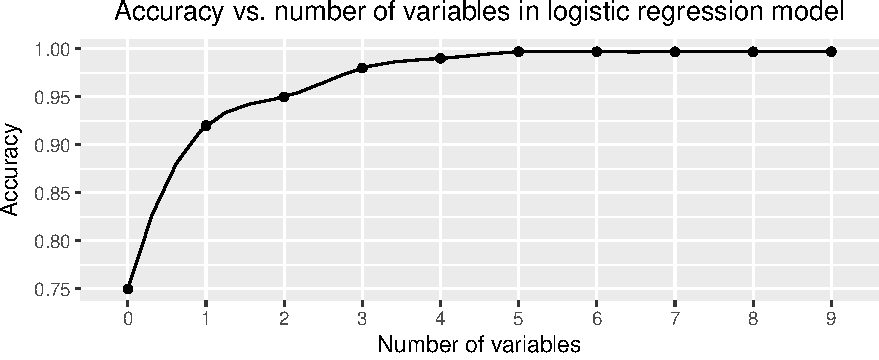
\includegraphics{logistic-regression_files/figure-latex/model_comparison-1} 

}

\caption{Accuracy vs. number of variables.}\label{fig:model_comparison}
\end{figure}

\section{Conclussions}\label{conclussions}

After our analysis, we have seen that two different aproaches are
possible in order to solve our classification problem, introduced at the
begining of this document. As showed above, we have studied two models:
a simpler one with two variables and 95\% of accuracy and a more complex
one with five variables and a 99\% of accuracy.

It is interesting to notice that the model with just two variables has
an easy explanation. Let's take a look at the Figure 2.

\begin{figure}[h]

{\centering 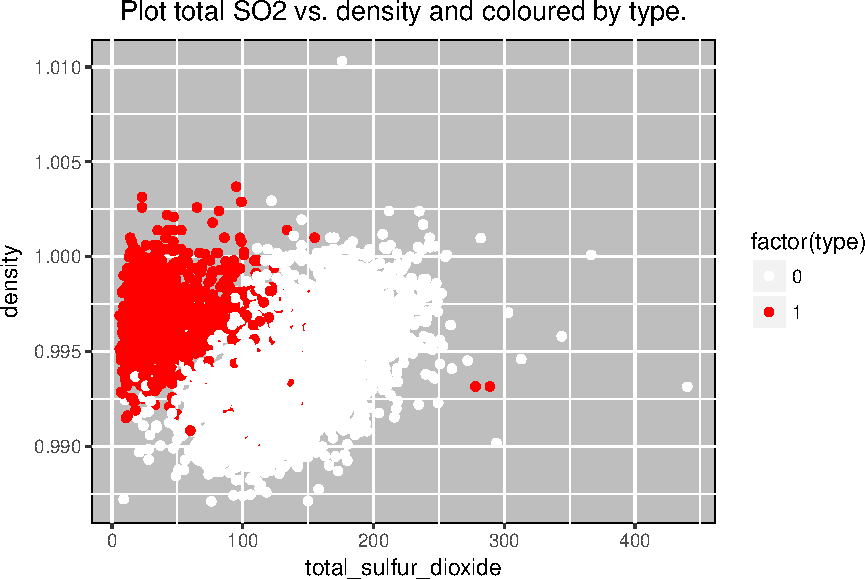
\includegraphics{logistic-regression_files/figure-latex/two_variables_plot-1} 

}

\caption{Total SO2 vs. density.}\label{fig:two_variables_plot}
\end{figure}

This plot shows the variables density and total SO2 but colored by type.
As we can see, it is clear that we have an almost perfect distinction
between red and white wines. That is why we are having such a great 95\%
accuracy in our simpler model.


\end{document}
